\section{Architectural Clones: A Step Toward Tactical Code Reuse}
\label{sec:Clones}
%\hl{The qualitative study conducted in this paper, motivated utilization of tactical clones as the minimum practical reuse granularity.}

The qualitative study we conducted motivated the utilization of tactical clones as an appropriate level of granularity in respect to code reusability. In order to illustrate the concepts of architectural or tactical clones, our qualitative study was followed by an exploratory study where we established a representative sample of these design clones. To assist, we developed a semi-automated process for retrieving candidate instances of tactic-related classes then detected code clones across these tactical files. 

The process of detecting tactical clones involves the following steps: (1) building a software repository, (2) extracting instances of architectural tactics, (3) extracting code clones across projects, and (4) manually inspecting the results to investigate our hypothesis that tactical clones are a practical granularity for architectural reuse.

\subsection{Building a software repository}

To build our repository of software systems, we preselected 37 open source projects with a high number of architectural tactics.

\begin{figure*}[!t]
\vspace{-1pt}
\centering
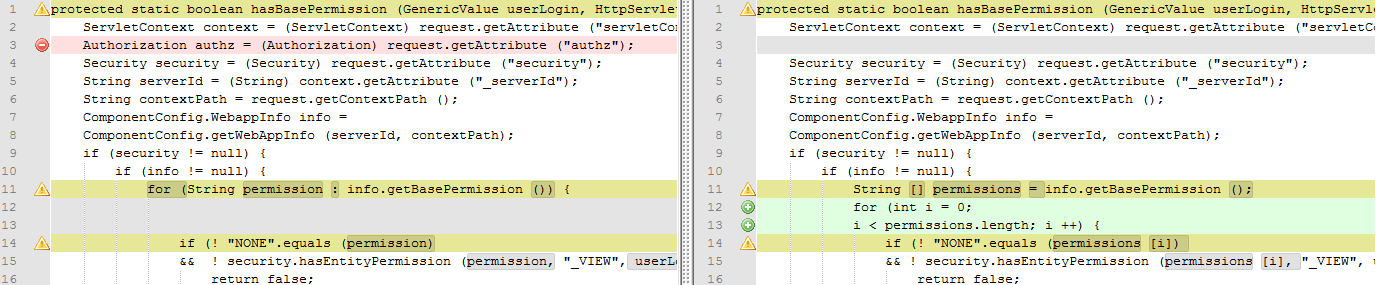
\includegraphics[width=0.9\linewidth]{./img/Permission}
\vspace{-6pt}
\caption{Tactical Clones Detected in Two different Projects}
\label{fig:Permission}
\vspace{-1pt}
\end{figure*}



\subsection{Extracting architectural tactics}
We utilized a previously developed tactic detection algorithm and tool~\cite{ICSE2012, FSE2014} to identify architectural tactics. These Tactic Detector's classifiers have been trained to find architectural tactics such as \textit{audit trail}, \textit{asynchronous method invocation}, \textit{authentication}, \textit{checkpointing and roll back}, \textit{Heartbeat}, \textit{role-based access control (RBAC)}, \textit{resource pooling}, \textit{scheduling}, \textit{ping echo}, \textit{hash-based method authentication}, \textit{kerberos} and \textit{secure session management}. Due to space constraints, we provide only an informal description of our tactic detection approach. However a more complete description of the approach, including its related formulas, may be found in previous publications~\cite{Dissertation, ICSE2012}. The tactic detection technique uses a set of classification techniques. These classifiers are trained using code snippets representing different architectural tactics, collected from hundreds of high-performance, open-source projects \cite{FSE2012,ICSE2012,Dissertation}. During the training phase, the classifier learns the terms (method and variable names as well as development APIs) that developers typically use to implement each tactic and assigns each potential indicator term a weight with respect to each type of tactic. The weight estimates how strongly an indicator term signals an architectural tactic. For instance, the term \emph{priority} is found more commonly in code related to the \emph{scheduling} tactic than in other kinds of code, and therefore the classifier assigns it a higher weighting with respect to scheduling. During the classification phase, the indicator terms are used to evaluate the likelihood that a given file implements an architectural tactic.

The accuracy of the Tactic Detector has been evaluated in several studies \cite{ICSE2012,FSE2014,Dissertation}. In a series of  experiments it was able to correctly reject approximately 77-100\% of non-tactical code classes (depending on tactic types); recall 100\% of the tactics-related classes with precision of 65\% to 100\% for most tactics tactics.  The recall for the authentication, audit trail and asynchronous method invocation was 70\% .

While this approach does not return perfectly precise results, it has a tuning parameter which enables us to only include the tactical files with higher prediction confidence in our analysis, which will significantly reduce the search space and assist with the task of retrieving candidate tactical clones.


%The final projects are listed in Table \ref{tab:ChosenProjects}. For each project we report its name, the number of classes in the system, the number of tactic types covered (maximum 13), number of candidate design patterns detected (maximum 20), and the final count of pattern/tactic overlaps as predicted by our automated tools.  As depicted in this table, most of the included projects provided coverage of 5 or more tactic types; however in order to ensure coverage of all the studied tactics, we included a couple of additional projects simply because they included the targeted tactic type, even though their overall tactic coverage was low.

%%%%%%%%%%%%%%%%%%%%%%%%%%%%%%


\subsection{Detecting Tactical Clones}
In order to detect architectural clones we used code clone detection techniques to identify reused tactical methods across different projects. We define the four types of tactical code clones by extending the definitions from Roy et al.~\cite{Roy:2008:NAD:1437898.1438600}.


\textbf{Type-1 tactical clones} are the simplest, representing identical tactical code except for variations in whitespace, comments, and layout to the type-4 clones, which are the most complex.


\textbf{Type-2 tactical clones} have variations in identifiers, types, whitespace, literals, layout, and comments, but are otherwise syntactically identical.

\textbf{Type-3 tactical clones} are tactical fragments which are copied and have modifications such as added or removed statements, variations in literals, identifiers, whitespace, layout and comments.


\textbf{Type-4 tactical clones}, are tactical code segments that perform the same computation, but have been implemented using different syntactic variants. 
%Concolic analysis ~\cite{Sen:2005:CCU:1081706.1081750} can be used to detect type-4 tactical clones~\cite{wcre2013}.


% Traditionally it has been used for software testing~\cite{Sen:2005:CCU:1081706.1081750}, code clone detection~\cite{wcre2013}, and vulnerability recognition~\cite{Chen:2014:CIB:2554850.2554875}.


In an extensive experiment we ran a leading clone detection tool Nicad~\cite{Roy:2008:NAD:1437898.1438600}, over the tactical code snippets from 37 projects. We chose Nicad for our analysis since it is a mature and refined tool which has demonstrated its effectiveness in previous research~\cite{roy2008empirical}.

\begin{table}[tbph]
\vspace{-10pt}
\caption{Discovered Tactical Clones Across 37 Projects.}
\label{tab:ChosenProjects}
\centering

%\begin{tabular}{|p{2.0cm}|p{2cm}|p{2.4cm}|}
  \begin{tabular}{ c | l | l }
\hline

\bfseries Tactic & \bfseries Number~of~Clones & \bfseries In~Total~Tactical~Files \\ \hline \hline
Audit & 50    & 352 \\ \hline
Authenticate & 151   & 252 \\\hline
Checkpointing & 8     & 138 \\ \hline
Ping Echo & 10    & 103 \\ \hline
Pooling & 1021  & 1073 \\ \hline
RBAC  & 436   & 477 \\ \hline
Scheduling & 76    & 117 \\ \hline
Secure Session & 249   & 299 \\ \hline
HeartBeat & 0     & 11 \\ \hline
Kerbrose & 0     & 21 \\
\end{tabular}%
\vspace{-10pt}
\end{table}

\subsection{Results}
Table~\ref{tab:ChosenProjects} shows tactics used in our study, as well as the number of tactical clones across projects. The last column of this table illustrates the total number of tactical files used in our analysis. The tactical clones were detected at the method level. While we could have detected tactical clones at the sub-method level, we realized that method level tactical clones are easier to comprehend and therefore easier to reuse for the developers. We do not report tactical clones within the same project since developers typically reuse the source code within a project. We were interested in the tactical clones reused across various projects so we could identify intrinsic and reusable tactical code snippets. As a result of our exploratory study we found several examples of identical tactical code snippets. While most of the clones were type 1, 2 and 3, we also had several examples of \textit{conceptually equivalent} tactical code snippets (type 4).

 Figure~\ref{fig:Permission} shows the source code for RBAC tactics across two different projects. In this example two developers in different systems have potentially created the same code snippets to implement the tactic. This example is one instance among several similar observations of tactical clones across different projects. This supports the hypothesis that tactical clones are an appropriate level of granularity in respect to code reusability. However, as stated in future work we plan to examine this hypothesis in set of developer studies.


%  This observation and several similar detected clones also support the hypothesis the fact that tactical clones are a more common granularity for code adoption and reuse.


